\chapter{实验与评估}
为了评估\tool{}的有效性,本文进行了一系列广泛的实验来解决三个关
键的研究问题。本章将首先设置三个实验问题,然后分别对每一个研究问题详细描述实验方法、数据集、评估指
标等,并充分分析实验结果。

\section{研究问题设置}
本文在评估部分研究了以下三个研究问题:
\begin{itemize}
	\item \textbf{RQ1(检测 CC 问题):\tool{}在检测 CC 问题方面的效果如何?}为了回答 RQ1,本研究利用章节\ref{3.4} 构建的CC 问题数据集,以评估\tool{} 检测CC问题的有效性,并通过基于抽样的人工验证过程确认其可靠性。
	\item \textbf{RQ2(分析不兼容更改):\tool{} 在分析不兼容更改方面的效果如何?}为了回答 RQ2,本研究从数据集中每个 CC 问题的错误信息中提取了破坏性API,从而评估分析不兼容更改的召回率,并通过样本验证进一步评估其精确率。
	\item \textbf{RQ3(解决实际问题):\tool{} 能否检测到真实场景中的 CC 问题并提供有效的修复建议?}为了回答 RQ3,本研究复现了 26个章节\ref{3.3} 中收集的真实世界中的 CC 问题,以评估 \tool{} 是否能够检测并修复这些实际的 CC 问题。
\end{itemize}

\section{RQ1:检测 CC 问题}
\subsection{实验设置}
\textbf{研究方法。}RQ1使用 \tool{} 检测了数据集中所有 23,866 个软件包组合的 CC 问题。每个组合\textit{(A, B)}包含应用软件包 \textit{A}来自 apt 仓库的预定义版本)和库软件包 \textit{B}通过 pip 安装的默认版本)。需要注意的是, \tool{} 并不会深入分析 API 调用链,这意味着如果 \textit{B}是 \textit{A}的传递依赖项但没有直接调用关系,这可能会导致漏报。然而,如果 \textit{A} 的某个依赖项 \textit{C} 调用了 \textit{B} 中的破坏性 API,则 \textit{A} 和 \textit{B} 的安装也可能会在系统中引入 CC 问题。因此,如果在 \textit{C} 和 \textit{B} 之间识别出 CC 问题,也会认为 \textit{A} 和 \textit{B} 之间存在 CC 问题。RQ1使用抽样人工验证来检查检测出问题的准确性。对于检测到的问题进行手动验证以确定其正确性。样本量通过有限总体校正法计算,确保样本能够准确代表整个数据集。RQ1将置信水平设定为 95\%,将误差范围设定为 5\%,这属于标准的统计阈值。

\textbf{评估指标。}基于章节\ref{3.4}构建的 CC 问题数据集,RQ1在评估中考虑了七个指标:(1) 已验证的真实正例 (VTP):由 \tool{} 报告且通过人工验证的 CC 问题;(2) 直接真实正例 (DTP):由 \tool{} 报告且在数据集中存在的 CC 问题;(3) 误报 (FP):由 \tool{} 报告但未通过人工验证的 CC 问题;(4) 漏报 (FN):数据集中存在但 \tool{} 未检测到的 CC 问题。基于上述四个指标,可以计算出精确率(Precision)、召回率(Recall)和 F1 分数(F1 Score),对应的计算公式如公式\ref{equ:1}、\ref{equ:2}和\ref{equ:3}所示。
\begin{equation}
	\label{equ:1}
	Precision = VTP / (VTP + FP)
\end{equation}
\begin{equation}
	\label{equ:2}
	Recall = DTP / (DTP + FN)
\end{equation}
\begin{equation}
	\label{equ:3}
	F1 Score =2 * Precision * Recall / ( Precision + Recall)
\end{equation}
其中精确率评估\tool{} 是否能够精准地检测 CC 问题。召回率评估\tool{} 检测所有 CC 问题的能力。F1 分数结合了精准率和召回率,取值在0~1之间,体现了综合性能。

\subsection{结果分析}
采用上述研究方法,\tool{}共报告了 3,689 个 CC 问题。需要注意的是,\tool{} 报告的许多问题在 CC 问题数据集构建过程中并未被识别,因为初始兼容性测试仅涉及库软件包的导入,这可能无法触发所有破坏性 API。从这些报告的问题中,RQ1抽取了 348 个案例进行人工验证。表\ref{tab:RQ4}显示了 RQ1 的实验结果。
\begin{table}[htbp]
	\centering
	\begin{threeparttable}
	\caption{\tool{}检测CC问题的有效性}
	\label{tab:RQ4}
	\begin{tabularx}{0.86\textwidth}{@{}ccccccccc@{}}
		\toprule
		\textbf{组}& \textbf{组合}& \textbf{\textit{VTP}} & \textbf{\textit{误报}} & \textbf{\textit{DTP}} & \textbf{\textit{漏报}} & \textbf{\textit{精确率}} & \textbf{\textit{召回率}} & \textbf{\textit{F1 分数}} \\ 
		\midrule
		G1    &  309   & 27   & 2   & 55   & 34  &  93.1 & 61.8  &  74.3  \\
		G2    &  472   & 44   & 1   & 225  & 36  &  97.8 & 86.2  &  91.6  \\
		G3    &  327   & 27   & 4   & 81   & 10  &  87.1 & 89.0  &  88.0  \\
		G4    &  1,214  & 100  & 14  & 669  & 8   &  87.7 & 98.8  &  92.9  \\
		G5    &  1,367  & 117  & 12  & 555  & 19  &  90.7 & 96.7  &  93.6  \\
		\midrule
		\textbf{总数/平均}  & 3,689  & 315 & 33 & 1,585 & 107 & 90.5 &  93.7 & 92.1   \\
		\bottomrule
	\end{tabularx}
	\end{threeparttable}
\end{table}
\tool{} 检测 CC 问题的精准率为 90.5\%,召回率为 93.7\%,F1 分数为 92.1\%。根据结果,RQ1可以得出结论,\tool{} 能够有效地检测 CC 问题。接下来,本节分别分析误报和漏报。

\subsubsection{误报分析}
本节总结了\tool{}误报的三大主要原因:
\begin{itemize}
	\item \textbf{(a) 未使用可选参数或额外参数列表(17/33):}在第三方软件包的演进过程中,移除函数中的可选参数或额外参数列表通常被视为一种后向不兼容更改。然而,当函数调用仅使用必选参数时,这种不兼容更改不会对其产生影响。在检测 CC 问题时,\tool{}查询依赖表时仅检查破坏性 API 的使用情况,而未考虑参数的使用情况,导致了误报的产生。
	\item \textbf{ (b) 用于赋值的破坏性函数 API(10/33):}当破坏性函数 API 用于赋值而未被调用时,不会触发 CC 问题。目前,依赖表仅存储 API 使用情况,而未考虑使用类型,这导致了误报的产生。例如,在应用软件包 “partd 1.11.1” \upcite{partd} 中,代码 \textit{decompress\_bytes = blosc.decompress} 将破坏性 API \textit{blosc.decompress} 赋值给 \textit{decompress\_bytes},而未调用它,因此不会引发 CC 问题。
	\item \textbf{ (c) 错误的破坏性 API(6/33):}在某些库软件包的某些版本中,API 提取未能捕获所有提供的 API 或提取的 API 名称与实际 API 调用名称不匹配。这导致兼容性表中存储了错误的破坏性 API,从而引发了这些误报。例如,在库软件包 “humanfriendly 10.0” \upcite{humanfriendly} 中,API 提取时将 API 名称识别为 \textit{humanfriendly.model.coerce\_boolean},而实际的 API 调用名称是 \textit{humanfriendly.coerce\_boolean}。
\end{itemize}

\subsubsection{漏报分析}
\tool{} 共产生了 107 个漏报,其中 59 个是由于依赖表未存储相应破坏性 API 的使用情况。在提取 API 使用情况时,\tool{} 主要检测了具有频繁 API 调用的 AST 节点,如 \textit{atom\_expr} 节点和 \textit{argument} 节点。其他节点中破坏性 API 的使用情况导致了这些漏报的产生。此外,一些破坏性 API 的使用情况并未出现在 *.py 文件中,例如,“pipdeptree 0.13.2-1build1” \upcite{pipdeptree} 和 “pip 23.1.2” \upcite{pip} 之间的破坏性 API 使用发生在 \textit{*.pyx} 文件中,而 \tool{} 无法分析 \textit{*.pyx} 或 \textit{*.pyc} 文件。其余 48 个漏报是由于兼容性表未存储这些案例中对应的破坏性 API。这主要是由于 API 提取失败或在分析不兼容更改时判定规则未涵盖所有不兼容更改场景。

\ignore{
\begin{tcolorbox}[boxrule=1pt,boxsep=1pt,left=2pt,right=2pt,top=2pt,bottom=2pt]
	\small
	\textcolor{red}{\faIcon{user-edit}} \noindent\textbf{RQ1结论:} 
	在本实验中,使用\tool{}对数据集中的23,866个软件包组合进行了CC问题检测。实验结果显示,\tool{}的精确率为90.5\%,召回率为93.7\%,F1分数为92.1\%,表明其有效性。尽管表现良好,\tool{}还存在误报和漏报,主要由于未充分分析参数依赖和API调用。误报常因API使用情况的错误判定而发生,漏报则由于关键API信息缺失或文件类型支持不足导致。未来通过改进API分析和扩展文件类型支持可以进一步提高\tool{}的检测精度和实用性。
\end{tcolorbox} 
}

\subsection{结论}
在本实验中,使用\tool{}对数据集中的23,866个软件包组合进行了CC问题检测。实验结果显示,\tool{}的精确率为90.5\%,召回率为93.7\%,F1分数为92.1\%,表明其有效性。尽管表现良好,\tool{}还存在误报和漏报,主要由于未充分分析参数依赖和API调用。误报常因API使用情况的错误判定而发生,漏报则由于关键API信息缺失或文件类型支持不足导致。未来通过改进API分析和扩展文件类型支持可以进一步提高\tool{}的检测精度和实用性。

\section{RQ2:分析不兼容更改}
\subsection{实验设置}
\textbf{研究方法。}RQ2 旨在评估 \tool{} 的核心组件——兼容性表,重点关注分析不兼容更改的有效性。为了评估精确率,RQ2根据兼容性表中每种不兼容更改模式的比例,对破坏性 API 进行分层随机抽样,并使用与 RQ1 相同的样本量计算方法。对于每个抽样的破坏性 API,安装库软件包的相应 apt 版本和 pip 版本,并手动验证调用该破坏性 API 是否会导致兼容性问题。为了评估召回率,RQ2验证了 CC 问题数据集中的破坏性 API 是否存在于兼容性表中。

\textbf{评估指标。}RQ2采用了六个评估指标:(1) 已验证的真实正例 (VTP):从兼容性表中抽样并通过人工验证的破坏性 API;(2) 直接真实正例 (DTP):在 CC 问题数据集中且存在于兼容性表中的破坏性 API;(3) 误报 (FP):从兼容性表中抽样但未通过人工验证的破坏性 API;(4) 漏报 (FN):存在于 CC 问题数据集中但不在兼容性表中的破坏性 API。基于这些指标,RQ2使用与 RQ1 相同的方法计算精确率和召回率。精确率评估 \tool{} 是否能够准确分析不兼容更改,而召回率评估 \tool{} 是否能够分析所有不兼容更改。
\subsection{结果分析}
图\ref{fig:RQ5-1}展示了\tool{}分析不兼容更改的精确率。整体来看,在抽样的 384 个破坏性 API 中,350 个通过了人工验证,34 个未通过,精确率为 91.1\%。漏报来自四类更改,包括 API 添加、API 删除、参数添加和可选参数添加。在 CC 问题数据集中共计 1,674 个破坏性 API,其中 1,644 个存在于兼容性表中,召回率为 98.2\%。根据实验结果,RQ2可以得出结论:\tool{} 能够有效地分析不兼容更改。\tool{}也存在一定程度的误报和漏报,接下来本节进行了详细的误报和漏报分析,以识别不兼容更改分析中的主要问题。
\begin{figure}[htbp]
	\centering
	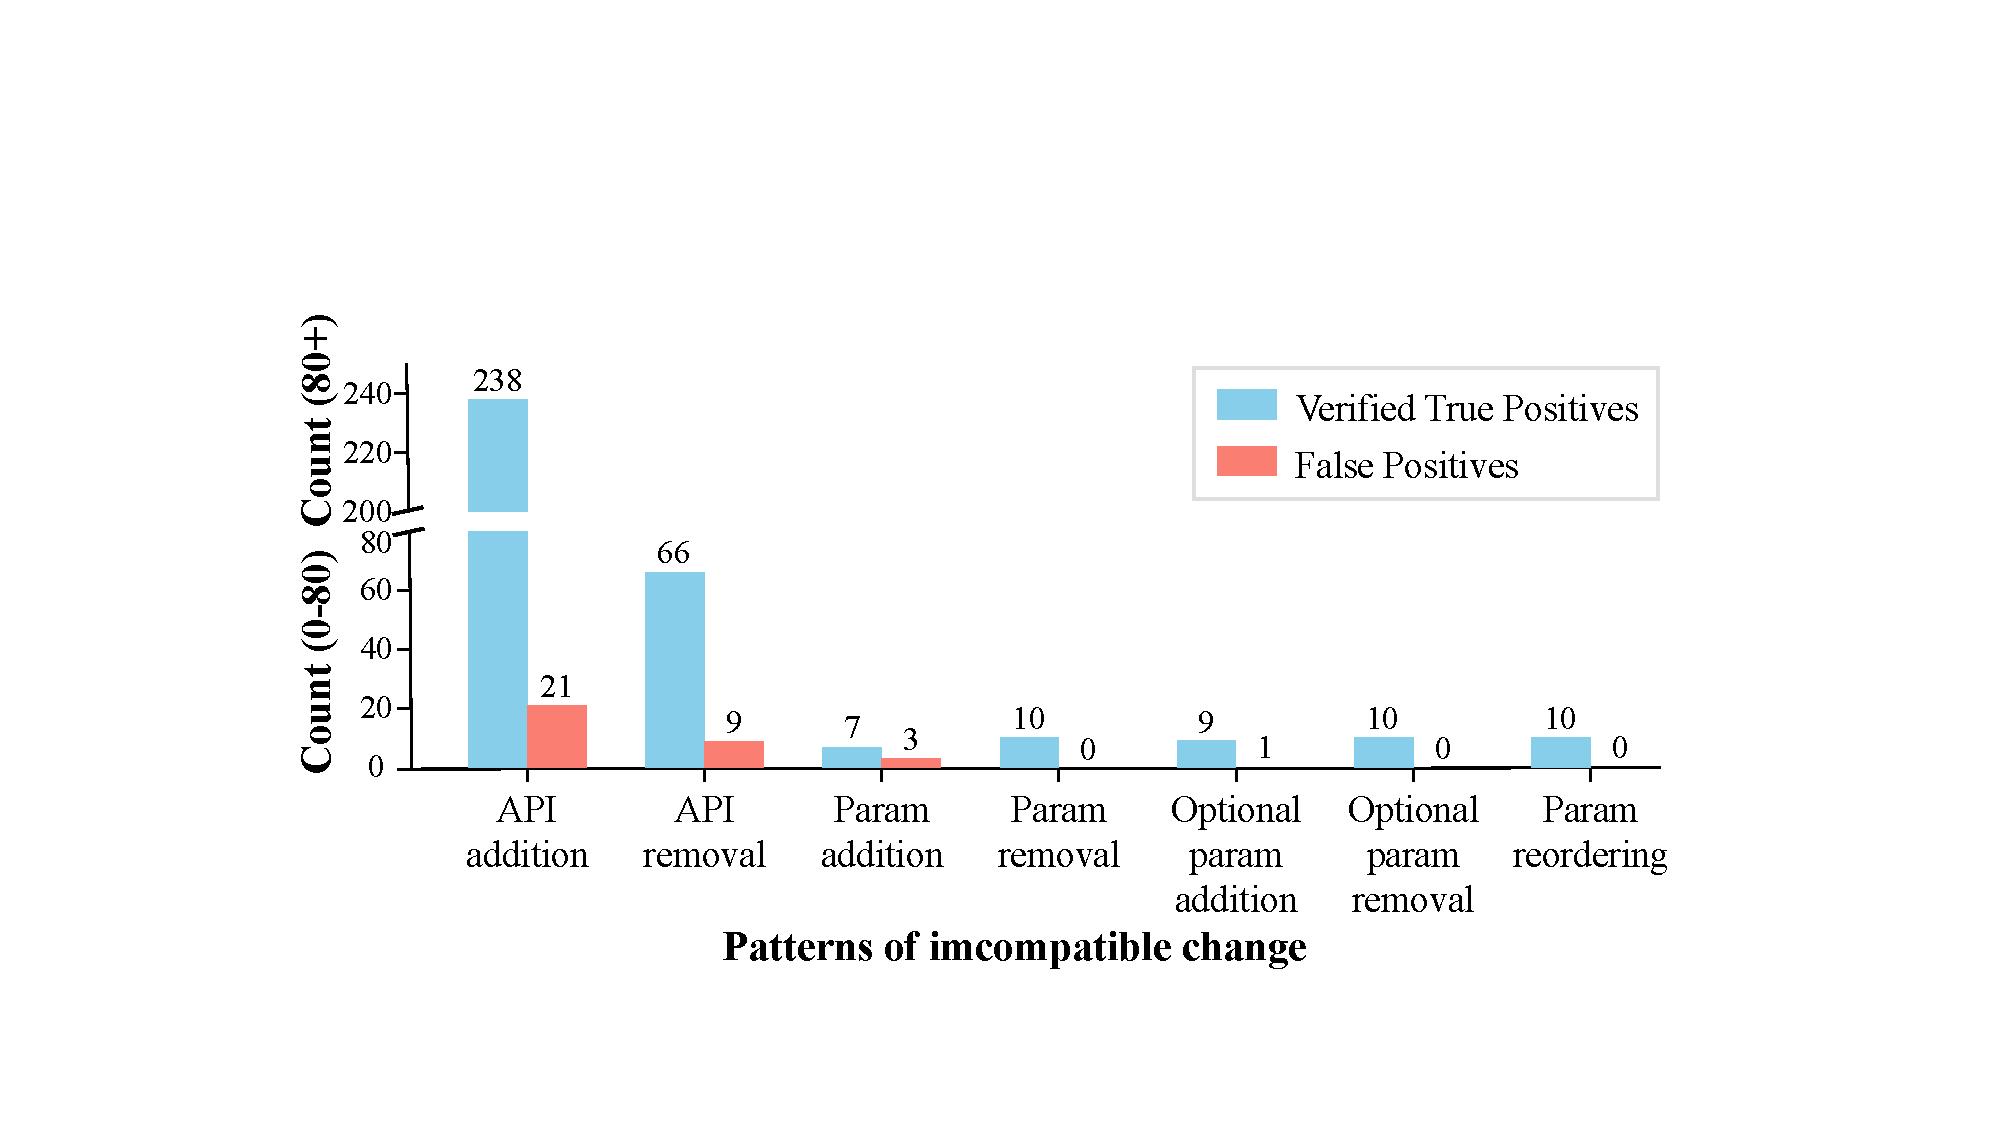
\includegraphics[width=\textwidth]{RQ2-1}
	\label{fig:RQ5-1}
	\caption{\tool{}分析不兼容更改的精确率}
\end{figure}

\ignore{
\begin{figure}[t]
	\centering
	\subfloat[分析不兼容更改的精确率]{
		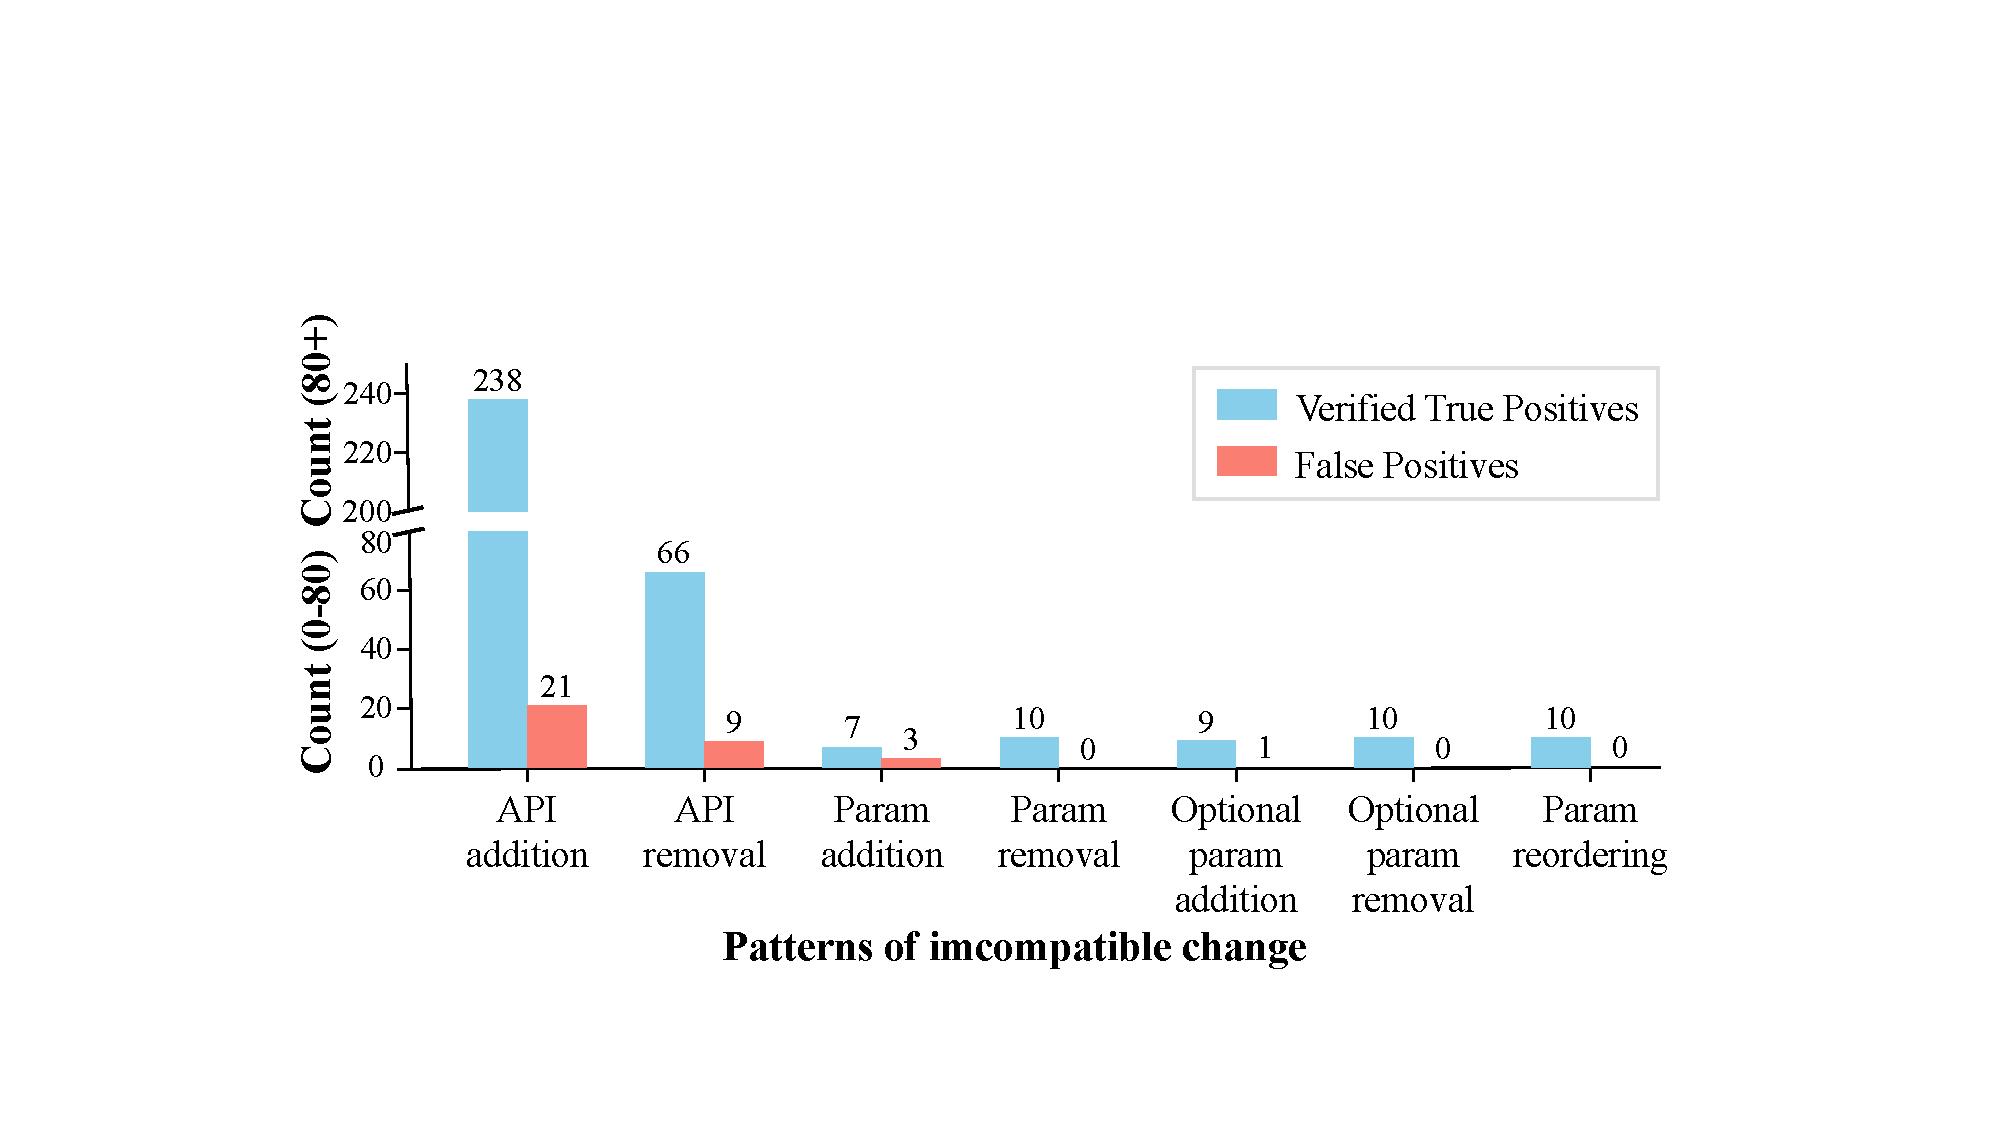
\includegraphics[width=\textwidth]{RQ2-1}
		\label{fig:RQ5-1}
	}\hspace{4em}
	\subfloat[分析不兼容更改的召回率]{
		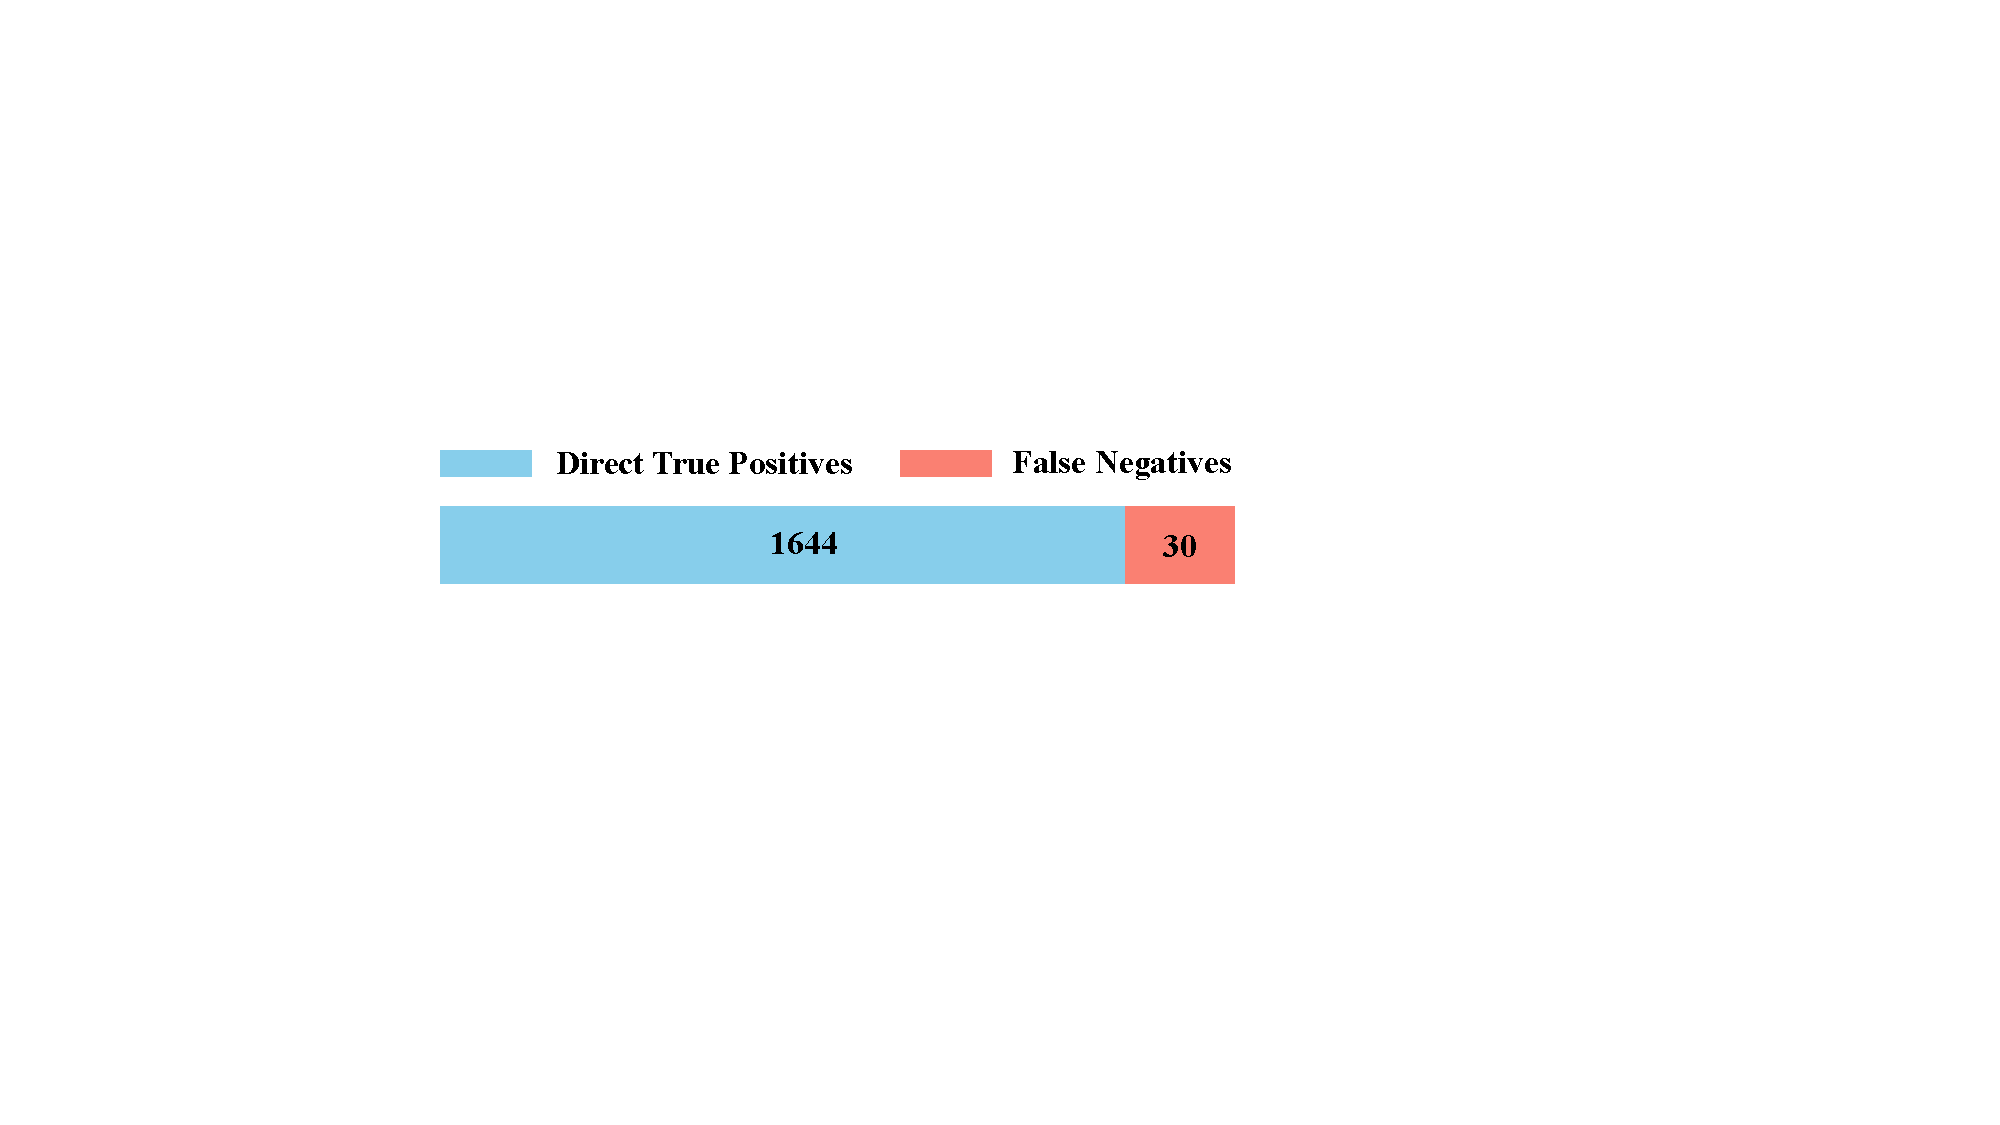
\includegraphics[width=.85\textwidth]{RQ2-2}
		\label{fig:RQ5-2}
	}
	\caption{RQ5的实验结果}
	\label{fig:RQ5}
	% \vspace{-2mm}
\end{figure}
}

\subsubsection{误报分析}
本节根据不兼容更改模式分别对误报进行分析:
\begin{itemize}
	\item \textbf{(a) API 添加和移删除(30/34):}这是最常见的误报类型,这两类中的误报主要是由于 API 提取过程未能提取所有 API。\tool{} 采用动态反射来提取 API,动态反射方法依赖于模块的完全加载但当 Python 解释器由于缺少必要的依赖项而加载特定模块时,\tool{}无法通过反射来获取这些模块的API。某些版本的库软件包未声明其所有依赖项,导致无法自动安装必要的依赖项。因此,依赖这些未安装依赖项的模块无法被导入,导致 API 丢失。
	\item \textbf{ (b) 参数添加(3/34):}该类别中的 3 个误报是由于添加的参数属于额外参数列表的一部分(例如,“xarray 0.15.0” 和 “xarray 2022.10.0” \upcite{xarray} 中的 \textit{xarray.open\_rasterio})。\tool{}的规则认为参数添加会导致前向不兼容更改和后向不兼容更改,因此\tool{}将其误判为同时影响前向和后向兼容性。但当参数被添加到参数列表时,它仅会导致后向不兼容更改。RQ2将这种对不兼容更改类型的误判视为误报。
	\item \textbf{ (c) 可选参数添加(1/34):}可选参数添加类别中的 1 个误报也是由于不兼容更改类型的误判导致的。这一问题出现在库软件包 “marshmallow” \upcite{marshmallow} 中\textit{ marshmallow.fields.Field} 类的构造函数中。新版本修改了该类,使其要求使用关键字参数,并将可选参数添加到了参数列表中。\tool{}将其报告为可选参数添加和后向不兼容更改。然而,这种更改应被视为 后向不兼容更改 和 前向不兼容更改,这导致了漏报。
\end{itemize}

\subsubsection{漏报分析}
所有漏报均是由于在构建兼容性表时的 API 提取步骤中遗漏了一些 API 引起的。这些遗漏主要与缺少必要的依赖项有关,导致无法导入相关模块,从而无法动态提取 API。此外,由于某些库软件包设计的复杂性和工具设计的局限性,\tool{} 无法提取相关的 API。

\ignore{
\begin{tcolorbox}[boxrule=1pt,boxsep=1pt,left=2pt,right=2pt,top=2pt,bottom=2pt]
	\small
	\textcolor{red}{\faIcon{user-edit}} \noindent\textbf{RQ2结论:} 
	RQ2评估了\tool{}在分析不兼容更改方面的有效性,在 95\% 的置信水平和 5\% 的误差范围下,结果显示其精确率为91.1\%,召回率达到了98.2\%。这表明\tool{}能够有效识别和分析不兼容更改,尽管存在一定比例的误报和漏报。误报主要是由于动态反射API提取失败,特别是当Python解释器因缺少依赖而无法加载模块时,以及对不兼容更改类型的误判。漏报主要因API提取过程中未能捕捉到所有API,通常与缺少的依赖项和模块导入失败相关。这些结果表明\tool{}目前在处理依赖复杂和动态环境时有一定局限性,未来可以通过改善API提取准确性和完善不兼容更改的分类方法进一步提高\tool{}的实用性和可靠性。
\end{tcolorbox} 
}
\subsection{结论}
RQ2评估了\tool{}在分析不兼容更改方面的有效性,在 95\% 的置信水平和 5\% 的误差范围下,结果显示其精确率为91.1\%,召回率达到了98.2\%。这表明\tool{}能够有效识别和分析不兼容更改,尽管存在一定比例的误报和漏报。误报主要是由于动态反射API提取失败,特别是当Python解释器因缺少依赖而无法加载模块时,以及对不兼容更改类型的误判。漏报主要因API提取过程中未能捕捉到所有API,通常与缺少的依赖项和模块导入失败相关。这些结果表明\tool{}目前在处理依赖复杂和动态环境时有一定局限性,未来可以通过改善API提取准确性和完善不兼容更改的分类方法进一步提高\tool{}的实用性和可靠性。

\section{RQ3:解决实际问题}
\subsection{实验设置}
\textbf{研究方法。}RQ3 利用\ref{3.3.1}中收集的真实世界CC问题来评估\tool{}在解决实际问题上的有效性。具体而言,本节首先深入分析每个问题的问题描述和错误信息,从中获取发生CC问题时相关的包和系统环境,然后,本节利用docker构建相互独立的环境尝试复现CC问题,当复现得到的错误信息和收集的错误信息一致时,认为该CC问题复现成功。对于每一个复现成功的CC问题,本节使用\tool{}进行检测,如果\tool{}报告了正确的CC问题,将根据\tool{}给出的修复建议进行修复,并验证是否修复成功。

\subsection{结果分析}
基于上述方法,RQ3成功复现了 26 个 CC 问题,并且 \tool{} 能够检测到所有这些问题。所有问题均列于表\ref{tab:issues} 中
此外,根据\tool{} 的建议,在导入应用软件包之前先从 apt 目录中导入库软件包,RQ3成功修复了所有 CC 问题。
无法复现的问题是问题\#6123796520\upcite{questions61237965},原因是开发者提供的环境信息不足。
% \begin{table}[t]
	% \centering
	% \caption{Effectiveness of \textit{Demian} in detecting real-world PA Issue.}
	% \label{tab:7}
	% \begin{tabularx}{\linewidth}{|c|l|l|l|c|}
		% \hline
		% \textbf{Issue ID} & \textbf{apt pkg} & \textbf{pip pkg} & \textbf{Incom. API} & \textbf{Detected} \\
		% \hline
		% *75244186 & scipy & numpy & numpy.int & \checkmark \\
		% \hline
		% *61237965 & pandas & numpy & \makecell[l]{testing. \\ decorators} & \checkmark \\
		% \hline
		% *76383191 & flask & jinja2 & escape & \checkmark \\
		% \hline
		% \#5154    & jinja2 & markupsafe & soft\_unicode & \checkmark \\
		% \hline
		% \multicolumn{4}{|c|}{Total Issues Detected} & 26/23 \\
		% \hline
		% \end{tabularx}
	% \end{table}
\begin{table}[htbp]
	\footnotesize
	%\scriptsize
	\centering
	\setlength\tabcolsep{2pt}     % horizental space
	\def\arraystretch{1.2}
	% \vspace{-2mm}
	\caption{RQ3的实验结果}
	\bgroup
	\definecolor{Status1}{HTML}{ff3300}
	\definecolor{Status2}{HTML}{1E90FF}
	\definecolor{Status3}{HTML}{336633}
	\definecolor{Status4}{HTML}{33ff99}
	\definecolor{Status5}{HTML}{993399}
	\definecolor{Status6}{HTML}{FF7F00}
	\definecolor{Status7}{HTML}{8E7111}
	\definecolor{Status8}{HTML}{878787}
	\definecolor{Status9}{HTML}{E535E5}
	\definecolor{Status10}{HTML}{35E54D}
	\begin{tabular}{|l|}
		% \toprule
		\hline
		\rowcolor[HTML]{9AFF99} 
		\multicolumn{1}{|c|}{\cellcolor[HTML]{9AFF99}\textbf{27 真实世界 CC 问题}} \\ \hline
		questions\#75244186{\color{Status1}$\spadesuit$}{\color{Status9}$\blacksquare$}{\color{Status10}$\blacksquare$}{\color{Status5}$\blacksquare$};
		questions\#61237965{\color{Status1}$\spadesuit$}{\color{Status7}$\blacksquare$};
		questions\#76383191{\color{Status1}$\spadesuit$}{\color{Status9}$\blacksquare$}{\color{Status10}$\blacksquare$}{\color{Status5}$\blacksquare$};
		\\
		\rowcolor[HTML]{EFEFEF}
		questions\#72593814{\color{Status1}$\spadesuit$}{\color{Status9}$\blacksquare$}{\color{Status10}$\blacksquare$}{\color{Status5}$\blacksquare$};
		questions\#74843336{\color{Status1}$\spadesuit$}{\color{Status9}$\blacksquare$}{\color{Status10}$\blacksquare$}{\color{Status5}$\blacksquare$};
		questions\#74411148{\color{Status1}$\spadesuit$}{\color{Status9}$\blacksquare$}{\color{Status10}$\blacksquare$}{\color{Status5}$\blacksquare$};
		\\
		questions\#74515643{\color{Status1}$\spadesuit$}{\color{Status9}$\blacksquare$}{\color{Status10}$\blacksquare$}{\color{Status5}$\blacksquare$};
		linode\_panel\#1{\color{Status2}$\clubsuit$}{\color{Status9}$\blacksquare$}{\color{Status10}$\blacksquare$}{\color{Status5}$\blacksquare$};
		ethz\_piksi\_ros\#234{\color{Status2}$\clubsuit$}{\color{Status9}$\blacksquare$}{\color{Status10}$\blacksquare$}{\color{Status5}$\blacksquare$};
		\\
		\rowcolor[HTML]{EFEFEF}
		gradio\#5154{\color{Status1}$\spadesuit$}{\color{Status9}$\blacksquare$}{\color{Status10}$\blacksquare$}{\color{Status5}$\blacksquare$};
		frr\#14816{\color{Status2}$\clubsuit$}{\color{Status9}$\blacksquare$}{\color{Status10}$\blacksquare$}{\color{Status5}$\blacksquare$};
		In0ri\#10{\color{Status2}$\clubsuit$}{\color{Status9}$\blacksquare$}{\color{Status10}$\blacksquare$}{\color{Status5}$\blacksquare$};
		gramine\#1142{\color{Status2}$\clubsuit$}{\color{Status9}$\blacksquare$}{\color{Status10}$\blacksquare$}{\color{Status5}$\blacksquare$};
		\\
		gsc\#121{\color{Status1}$\spadesuit$}{\color{Status9}$\blacksquare$}{\color{Status10}$\blacksquare$}{\color{Status5}$\blacksquare$};
		PyDodge\#24{\color{Status2}$\clubsuit$}{\color{Status9}$\blacksquare$}{\color{Status10}$\blacksquare$}{\color{Status5}$\blacksquare$};
		kasm-dof-workspace\#9{\color{Status2}$\clubsuit$}{\color{Status9}$\blacksquare$}{\color{Status10}$\blacksquare$}{\color{Status5}$\blacksquare$};
		linkml\#966{\color{Status2}$\clubsuit$}{\color{Status9}$\blacksquare$}{\color{Status10}$\blacksquare$}{\color{Status5}$\blacksquare$};
		\\
		\rowcolor[HTML]{EFEFEF}
		quart\#171{\color{Status1}$\spadesuit$}{\color{Status9}$\blacksquare$}{\color{Status10}$\blacksquare$}{\color{Status5}$\blacksquare$};
		LittlePaimon\#283{\color{Status2}$\clubsuit$}{\color{Status9}$\blacksquare$}{\color{Status10}$\blacksquare$}{\color{Status5}$\blacksquare$};
		fprime-tools\#48{\color{Status2}$\clubsuit$}{\color{Status9}$\blacksquare$}{\color{Status10}$\blacksquare$}{\color{Status5}$\blacksquare$};
		taipy\#255{\color{Status2}$\clubsuit$}{\color{Status9}$\blacksquare$}{\color{Status10}$\blacksquare$}{\color{Status5}$\blacksquare$};
		\\
		stable-diffusion-webui\#231{\color{Status1}$\spadesuit$}{\color{Status9}$\blacksquare$}{\color{Status10}$\blacksquare$}{\color{Status5}$\blacksquare$};
		mkchromecast\#451{\color{Status2}$\clubsuit$}{\color{Status9}$\blacksquare$}{\color{Status10}$\blacksquare$}{\color{Status5}$\blacksquare$};
		InstallScript\#396{\color{Status2}$\clubsuit$}{\color{Status9}$\blacksquare$}{\color{Status10}$\blacksquare$}{\color{Status5}$\blacksquare$};
		\\
		\rowcolor[HTML]{EFEFEF}
		cserbot\#9688{\color{Status2}$\clubsuit$}{\color{Status9}$\blacksquare$}{\color{Status10}$\blacksquare$}{\color{Status5}$\blacksquare$};
		fact\_CORE\#858{\color{Status2}$\clubsuit$}{\color{Status9}$\blacksquare$}{\color{Status10}$\blacksquare$}{\color{Status5}$\blacksquare$};
		frr\#14820{\color{Status4}$\diamondsuit$}{\color{Status9}$\blacksquare$}{\color{Status10}$\blacksquare$}{\color{Status5}$\blacksquare$};
		\\
		\hline
		% \\ \bottomrule
		\multicolumn{1}{l}{{\color{Status1}$\spadesuit$}: 来自Stack overflow的CC问题; }\\
		\multicolumn{1}{l}{{\color{Status2}$\clubsuit$}: 来自Github的CC问题;} \\
		\multicolumn{1}{l}{{\color{Status4}$\diamondsuit$}: 来自Github讨论区的CC问题;}\\
		\multicolumn{1}{l}{{\color{Status9}$\blacksquare$}: 成功复现的CC问题;}\\
		\multicolumn{1}{l}{{\color{Status7}$\blacksquare$}:未能成功复现的CC问题;}\\
		\multicolumn{1}{l}{{\color{Status10}$\blacksquare$}:  \tool{}检测成功的CC问题;}\\
		\multicolumn{1}{l}{{\color{Status5}$\blacksquare$}:\tool{}修复成功的CC问题.}\\
	\end{tabular}
	\egroup
	% \vspace{-2mm}
	\label{tab:issues}
\end{table}

\textbf{案例分析。}许多 CC 问题困扰着社区内的开发者,其中 gradio 的 Issue \#5154 \upcite{gradio_issue_5154} 就是一个例子。该开发者在运行 gradio 程序时遇到了应用软件包 “jinja2” 与库软件包 “markupsafe” 之间的兼容性问题。
\begin{figure}[t]
	\centering
	\subfloat[gradio 的 Issue \#5154的错误信息]{
		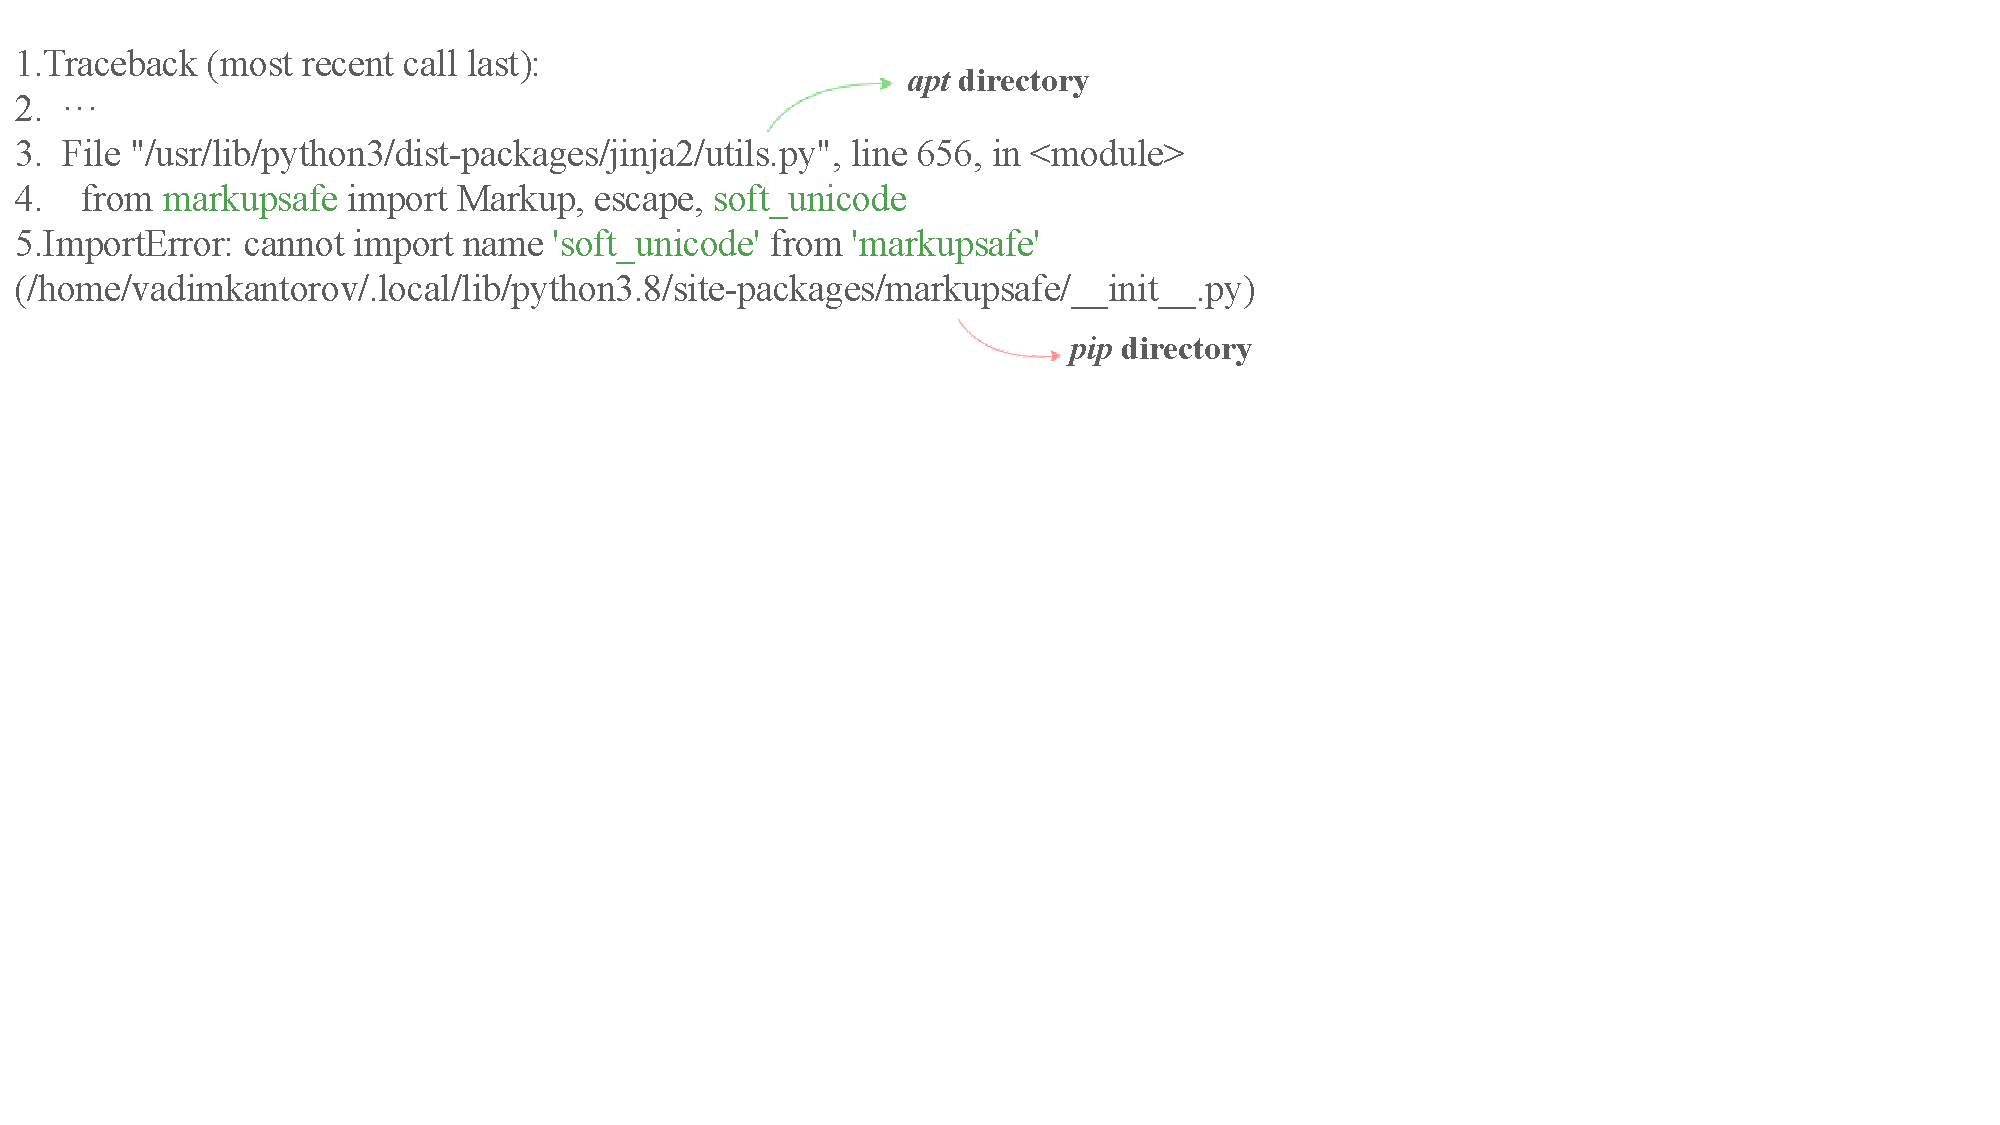
\includegraphics[width=.95\textwidth]{RQ3}
		\label{fig:RQ6-1}
	}\hspace{4em}
	\subfloat[gradio 的 Issue \#5154的API导入链]{
		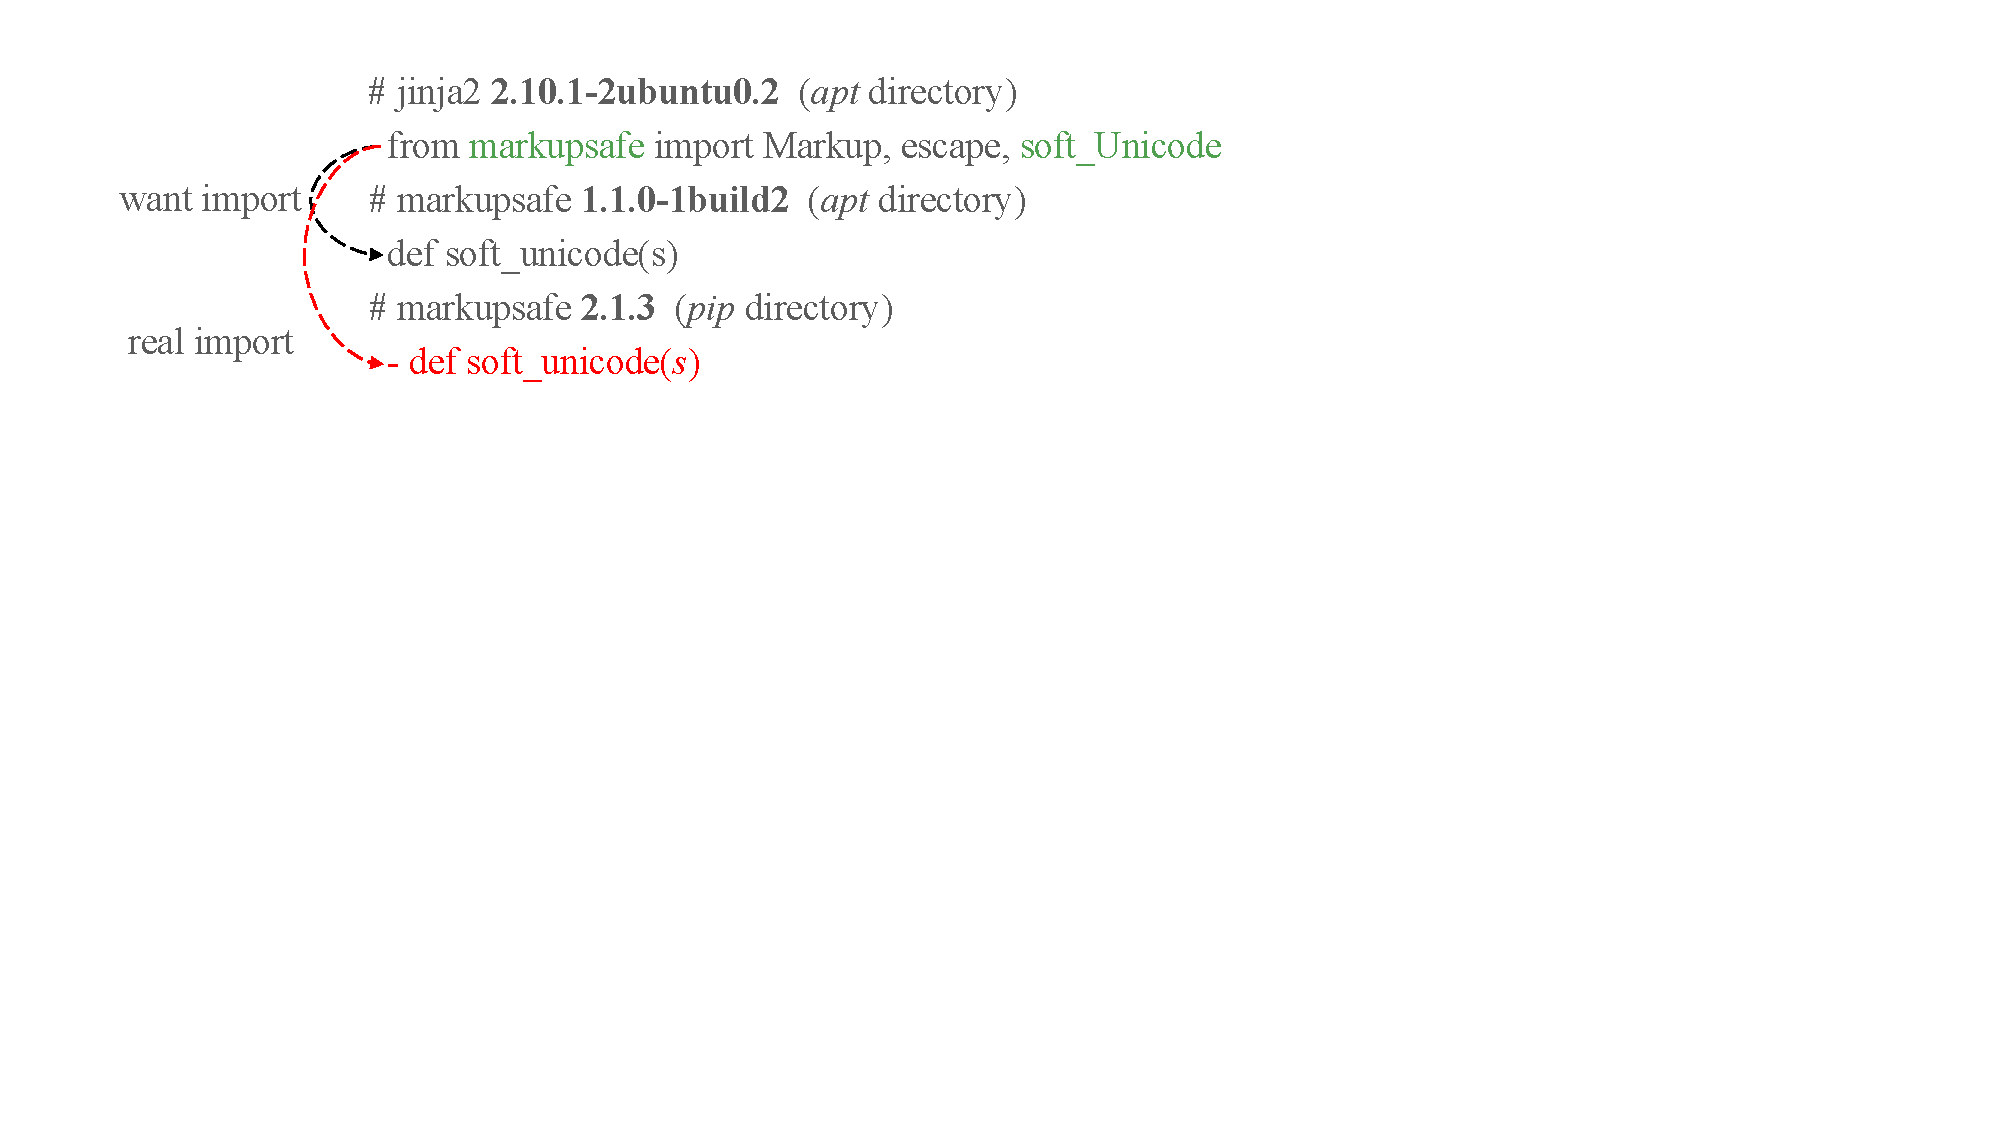
\includegraphics[width=.85\textwidth]{RQ3 import chain}
		\label{fig:RQ6-2}
	}
	\caption{一个真实世界CC问题案例}
	\label{fig:RQ6}
	% \vspace{-2mm}
\end{figure}
图 \ref{fig:RQ6-1}  显示了该问题回溯信息的关键部分,说明了来自 apt 目录的 “jinja2” 在尝试从 pip 目录中的 “markupsafe” 导入 \textit{soft\_unicode} 函数时遇到了错误。此外,图 \ref{fig:RQ6-2} 详细展示了 API 导入链,说明了 apt 目录中的 “jinja2 2.10.1-2ubuntu0.2” 试图从 apt 目录中的 “markupsafe 1.1.0-1build2” 导入 \textit{soft\_unicode} 函数,但 Python 解释器实际从 pip 目录中的 “markupsafe 2.1.3” 导入了该函数。但 2.1.3 版本删除了该属性,从而导致了该问题的发生。最终,开发者通过将 pip 目录中的库软件包 “markupsafe” 降级至支持 \textit{soft\_unicode} 的版本来解决了该问题。\tool{} 建议指定从 apt 目录中导入库软件包 “markupsafe”,这可以帮助用户避免在 pip 目录中重新安装兼容版本的 “markupsafe”,从而更轻松地解决该问题。此外,包管理器并未向用户提供该问题的任何警告,而 \tool{} 能够在软件包安装时预测到该问题。

\ignore{
\begin{tcolorbox}[boxrule=1pt,boxsep=1pt,left=2pt,right=2pt,top=2pt,bottom=2pt]
	\small
	\textcolor{red}{\faIcon{user-edit}} \noindent\textbf{RQ3结论:} 
	在RQ3中,本节评估了\tool{}在处理实际世界的CC问题中的有效性。针对26个复现的真实世界CC问题,\tool{}成功检测并修复了所有这些问题。这证明了\tool{}不仅能够准确识别和报告CC问题,还能提供有效的修复建议。特别是在处理像gradio Issue \#5154这样的复杂案例时,\tool{}展示了其能力,通过建议从apt目录导入库软件包“markupsafe”,帮助开发者避免不必要的降级操作。评估结果证明\tool{}在解决实际应用上的有效性和可用性,能够为开发者在遇到依赖冲突时提供直接和实用的解决方案。
\end{tcolorbox} 
}
\subsection{结论}
在RQ3中,本节评估了\tool{}在处理实际世界的CC问题中的有效性。针对26个复现的真实世界CC问题,\tool{}成功检测并修复了所有这些问题。这证明了\tool{}不仅能够准确识别和报告CC问题,还能提供有效的修复建议。特别是在处理像gradio Issue \#5154这样的复杂案例时,\tool{}展示了其能力,通过建议从apt目录导入库软件包“markupsafe”,帮助开发者避免不必要的降级操作。评估结果证明\tool{}在解决实际应用上的有效性和可用性,能够为开发者在遇到依赖冲突时提供直接和实用的解决方案。

\section{讨论}
本节分别讨论了本研究的局限性和可推广性。
\subsection{局限性}
首先,\tool{} 检测 CC 问题,并建议用户在导入应用软件包之前先从 apt 仓库中导入兼容的库软件包。然而,依赖于应用软件包的用户程序不一定会受到 CC 问题的影响。这是因为用户程序可能并未调用破坏性 API。要判断用户程序是否会因 CC 问题而遇到错误,需要进行在线程序分析以获取 API 调用链。目前,为了降低部署开销,\tool{}未进行在线程序分析。其次,一些跨仓库兼容性问题与本地模块和二进制库有关,而 \tool{} 当前无法解决这些问题。这是因为 \tool{} 当前的程序分析集中在 Python 语言,无法分析此类模块的 API 兼容性。本研究的工作重点是解决 Python 源代码级别的跨仓库第三方软件包兼容性问题,这已覆盖了用户遇到的大部分不兼容性问题。未来的工作将考虑上述局限性以优化 \tool{},并且应在实际开发环境中使用该技术进行长期评估,与此同时,未来将开展用户研究以提升 \tool{} 的可用性。
\subsection{推广性}
评估结果表明,\tool{} 能够有效解决 Ubuntu 系统与 Python 语言之间的 CC 问题。本研究还发现在其他 Linux 发行版生态系统和其他动态编程语言生态系统(例如 CentOS、Ruby)中存在类似的 CC 问题,并且这些问题的根本原因是一致的。因此,\tool{}的整体框架也适用于其他生态系统。然而,分析软件包兼容性的方法并不通用于不同语言的软件包。\tool{}通过分析不兼容的 API 来确定兼容性,但由于不同语言中 API 的实现方式各不相同,难以创建一个通用的方法来分析所有语言的第三方软件包兼容性。未来的研究应探索更通用的兼容性分析方法,以解决更多生态系统中的 CC 问题。

\section{本章小结}
本章深入探讨\tool{}解决跨软件生态的兼容性方面的有效性。通过一系列精心设计的评估实验和分析,本章探讨了\tool{}在检测、预测和修复CC问题方面的实际应用价值。本章首先通过三个研究问题详细探讨了\tool{}在检测CC问题,分析不兼容的更改和解决真实世界CC问题的有效性。在RQ1中,本章发现\tool{}能够有效的检测CC问题,精确率达到90.5\%,召回率达到93.7\%。在RQ2中,本章发现\tool{}在分析不兼容更改方面表现出较高的有效性,精确率达到91.1\%,召回率达到98.2\%。在RQ3中,本章发现\tool{}能够检测和修复全部26个被复现的真实世界CC问题,体现了工具在真实世界场景下的优秀可用性。最后,本章从局限性和推广性两方面对\tool{}进一步讨论,为后续的工具优化和相关研究工作提供了基础。